\documentclass{beamer}
%
% Choose how your presentation looks.
%
% For more themes, color themes and font themes, see:
% http://deic.uab.es/~iblanes/beamer_gallery/index_by_theme.html
%
\mode<presentation>
{
  \usetheme{default}      % or try Darmstadt, Madrid, Warsaw, ...
  \usecolortheme{default} % or try albatross, beaver, crane, ...
  \usefonttheme{default}  % or try serif, structurebold, ...
  \setbeamertemplate{navigation symbols}{}
  \setbeamertemplate{caption}[numbered]
} 

\usepackage[english]{babel}
\usepackage[utf8x]{inputenc}
\usepackage{wrapfig}
\usepackage{ amssymb }
\usepackage{ dsfont }
\usepackage{ fontawesome }

\title[ICLR zapłata]{Selected ICLR 2017 Papers}
\author{Agnieszka Pocha}
\institute{Jagiellonian University}
\date{19.05.2017, Kraków}

\begin{document}

\begin{frame}
  \titlepage
\end{frame}

% Uncomment these lines for an automatically generated outline.
\begin{frame}{Outline}
 \tableofcontents
\end{frame}

\section{Designing Neural Network Architectures using Reinforcement Learning}


\begin{frame}{Designing Neural Network Architectures using Reinforcement Learning}
  Bowen Baker, Otkrist Gupta, Nikhil Naik, Ramesh Raskar

  \vspace{0.1in}

  \begin{block}{Abstract}
  Designing NN architectures is slow and laborious. We would like to have an automatic and successful method to do it for us.\vspace{0.05in}
  Authors introduce MetaQNN - a \textbf{reinforcement learning method} based on \textbf{Q-learnig} algorithm that finds highly performing architectures.\vspace{0.05in}
  Their models:
  \begin{itemize}
  \item beat on CIFAR, MNIST \& SVHN best performing models that share similar architecture
  \item compare well with state-of-the-art models
  \item are suitable for transfer learning
  \end{itemize}
  Moreover, authors show that their method is stable.

  \end{block}
\end{frame}


\begin{frame}{Shortly}
  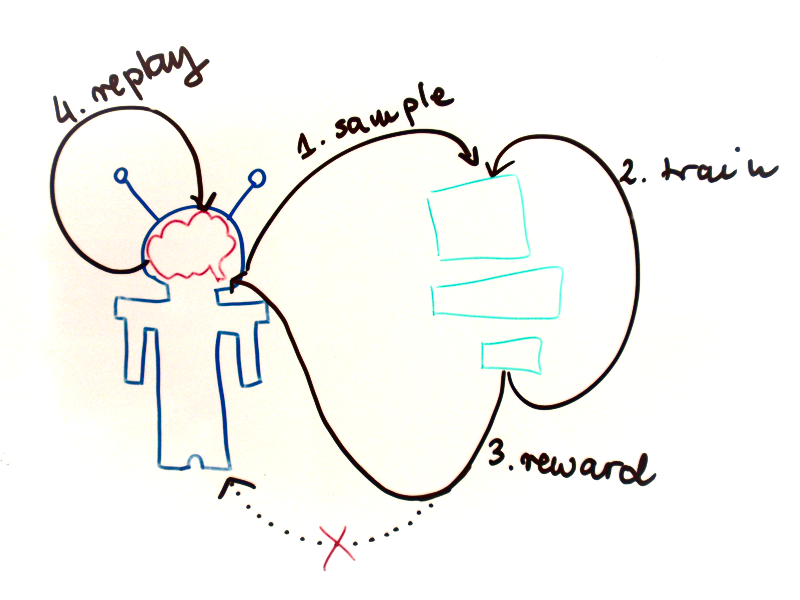
\includegraphics[width=0.9\textwidth]{model.png}

  Learning agent sequentially chooses CNN layers using \textbf{Q-learnig} with an \textbf{$\epsilon$-greedy exploration strategy} and \textbf{experience replay}.
\end{frame}


\begin{frame}{$\epsilon$-greedy exploration strategy}
  Choose what you think is the best option with probability $1-\epsilon$ and choose a random action with probability $\epsilon$.

  \begin{center}
  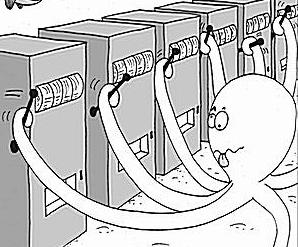
\includegraphics[width=0.6\textwidth]{exploration.jpg}
  \end{center}

  \begin{center}
  \begin{tiny}
  \url{http://research.microsoft.com/en-us/projects/bandits/}  
  \end{tiny}
  \end{center}
\end{frame}


\begin{frame}{Q-learnig}
  Let $\mathcal{S}$ - state space, $\mathcal{U}$- action space, $\mathcal{U}(s_i) \in \mathcal{U}$ - actions possible while in state $s_i$.
  \vskip0.1in
  In an environment with stochastic transitions, an agent in state $s_i$ taking some action $u \in \mathcal{U}$ will \textbf{transition} to state $s_j$ with probability $p_{s'|s, u}(s_j | s_i, u)$ which may be unknown to the agent.
  \vskip0.1in
  At each timestep $t$, the agent is given a \textbf{reward} $r_t$, dependent on the transition from state $s$ to $s'$ and action $u$. The reward may also be stochastic according to a distribution $p_{r|s', s, u}$.
  \vskip0.1in
  The agent's \textbf{goal} is to maximize the \textbf{total expected reward} over all possible trajectories, i.e. $max_{\tau_i \in \tau R_{\tau_i}}$, where the total expected reward for a trajectory $\tau_i$ is

  \begin{center}
  $R_{\tau_i} = \Sigma_{(s, u, s') \in \tau_i} \mathds{E}_{r|s, u, s'}[r|s, u, s']$
  \end{center}
\end{frame}


\begin{frame}{Q-learnig}
  Let $\mathcal{S}$ - state space, $\mathcal{U}$- action space, $\mathcal{U}(s_i) \in \mathcal{U}$ - actions possible while in state $s$.

  \begin{center}
  $R_{\tau_i} = \Sigma_{(s, u, s') \in \tau_i} \mathds{E}_{r|s, u, s'}[r|s, u, s']$
  \end{center}

  The number of possible trajectories makes the problem untractable, therefore we define the maximization problem recursively in terms of subproblems as follows: for any state $s_i \in S$ and subsequent action $u \in \mathcal{U}(s_i)$, we define the \textbf{maximum total expected reward} to be $Q^*(s_i, u)$. The recursive maximization equation, which is known as \textbf{Bellman's Equation}, can be written as:

  \begin{center}
  $Q^*(s_i, u) = \mathds{E}_{s_j|s_i, u}[ \mathds{E}_{r|s_i, u, s_j}[r|s_i, u, s_j] + \gamma max_{u' \in \mathcal{U}(s_j)} Q^*(s_j, u') ]$ 
  \end{center}

  We usually cannot solve it analytically but we can define an \textbf{iterative update}.
\end{frame}


\begin{frame}{Q-learning}
  \begin{itemize}
  \item \textbf{model-free}
  \item \textbf{off-policy}
  \item two parameters:
  \begin{itemize}
  \item $\alpha$ - \textbf{learning rate}
  \item $\lambda$ - \textbf{discount factor} (weight given to short term rewards over future rewards)
  \end{itemize}
  \end{itemize}
  
  Here:
  \begin{itemize}
  \item \textbf{action} - choosing next layer along with its parameters (size, stride...)
  \item \textbf{state} - the current state of the network topology
  \item \textbf{reward} - performance on validation set (5K samples, with unchanged class distribution)
  \end{itemize}
\end{frame}


\begin{frame}{Experience replay}
  Use single experience multiple times for an iterative update.
  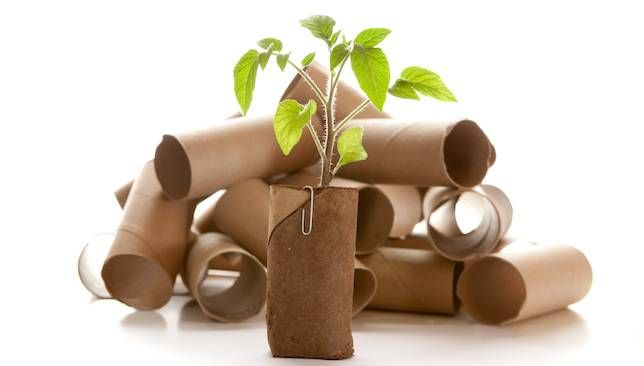
\includegraphics[width=\textwidth]{reuse.jpg}\\
  \begin{tiny}
  \url{https://www.shutterstock.com/image-photo/empty-toilet-paper-roll-recycled-seedling-134967662?src=ijY4nrNlx43dUDT2n_Cjsw-1-4}
  \end{tiny}
\end{frame}


\begin{frame}{Shortly (again)}
  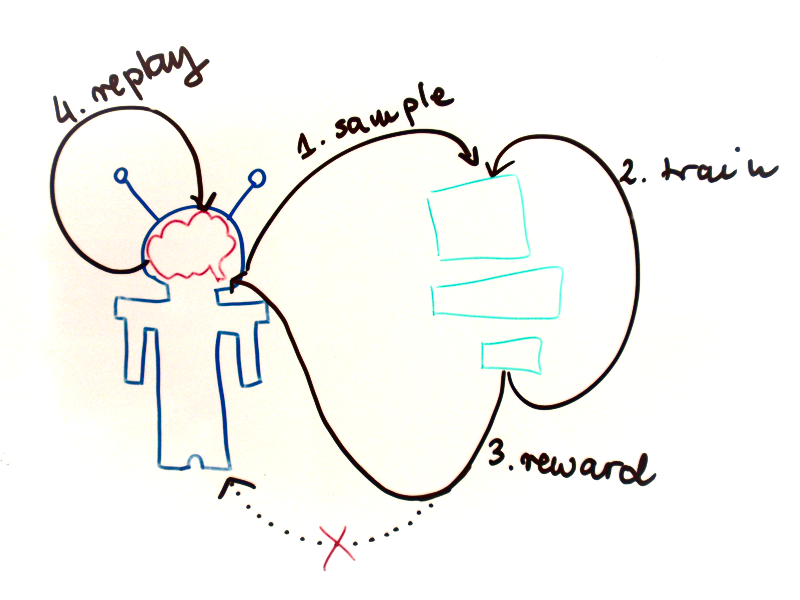
\includegraphics[width=0.9\textwidth]{model.png}

  Learning agent sequentially chooses CNN layers using \textbf{Q-learnig} with an \textbf{$\epsilon$-greedy exploration strategy} and \textbf{experience replay}.
\end{frame}


\begin{frame}{Training models}
  Models were trained in an aggresive fashion (stop this violence!) what made the process less costly.
  \begin{itemize}
  \item dropout every 2 layers
  \item 20 epochs
  \item Adam
  \item batch size 128
  \item learning rate 0.001 reduced by a factor of 0.2 every 5 epochs
  \item Xavier initialization (Glorot \& Bengio 2010)
  \end{itemize}

  \textbf{Time:} 8-10 days for each dataset on 10 NVIDIA GPUs (GMUM needs more GPUs).
\end{frame}


\begin{frame}{Again same picture but now we should understand it completely}
  \begin{center}
  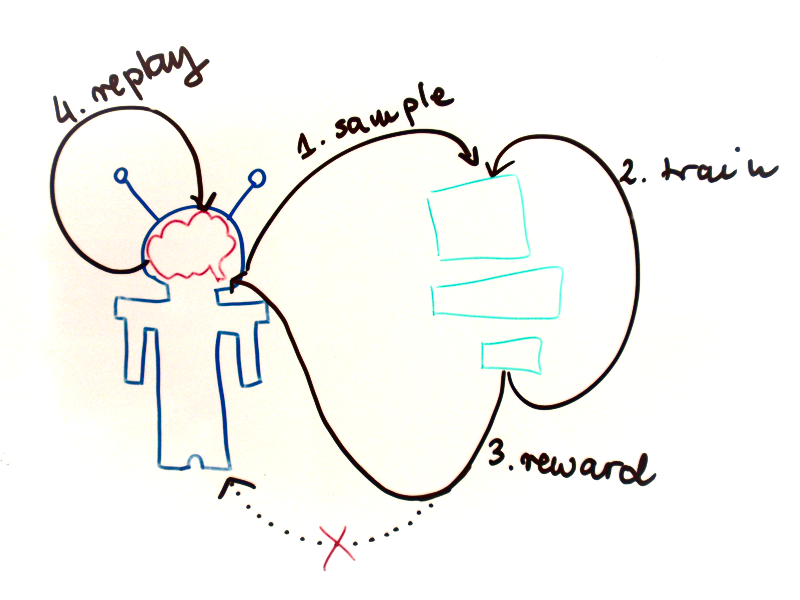
\includegraphics[width=0.7\textwidth]{model.png}  
  \end{center}
  
  Learning agent sequentially chooses CNN layers using \textbf{Q-learnig} with an \textbf{$\epsilon$-greedy exploration strategy} and \textbf{experience replay}.
\end{frame}

\begin{frame}{Experiments}
It grows! It means that the architectures chosen greedily/later (exploitation) are better than those randomly sampled (exploration) - the agent has learned something.
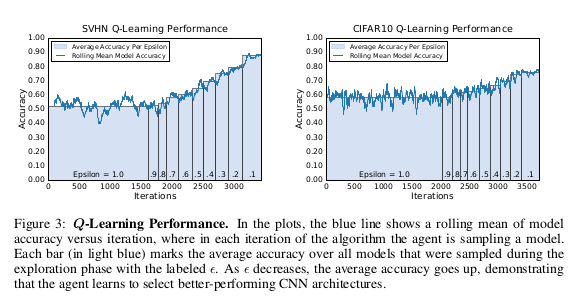
\includegraphics[width=\textwidth]{experiments.png}
\end{frame}

\begin{frame}{Experiments}
It learns! It means that the architectures chosen greedily/later (exploitation) are better than those randomly sampled (exploration) - the agent has learned something.
\begin{center}
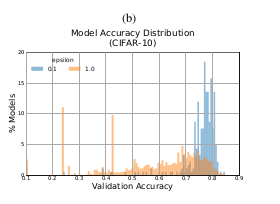
\includegraphics[width=0.9\textwidth]{exp2.png}
\end{center}
\end{frame}

\begin{frame}{Results}
After short training all those architectures 10 best were chosen and well tuned. Finally, 5 best were chosen to become ensemble.
\vskip0.1in
\begin{itemize}
  \item beat on CIFAR, MNIST \& SVHN best performing models that share similar architecture
  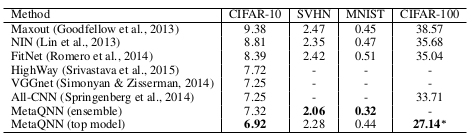
\includegraphics[width=0.8\textwidth]{best_on_similar.png}
  \end{itemize}
\end{frame}

\begin{frame}{Results}
  \begin{itemize}
  \item compare well with state-of-the-art models
  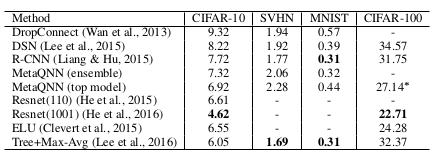
\includegraphics[width=0.9\textwidth]{state_art.png}
  \item are suitable for transfer learning
  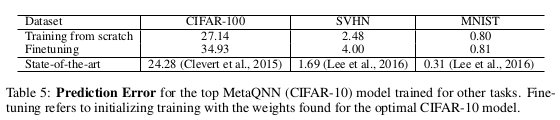
\includegraphics[width=0.9\textwidth]{transfer.png}
  \end{itemize}
\end{frame}

\begin{frame}{Results}
  \begin{itemize}
  \item stability
  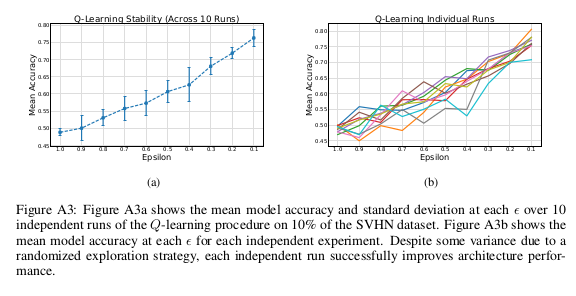
\includegraphics[width=0.9\textwidth]{stability.png}
  \end{itemize}
\end{frame}




\begin{frame}{My problem with this paper}
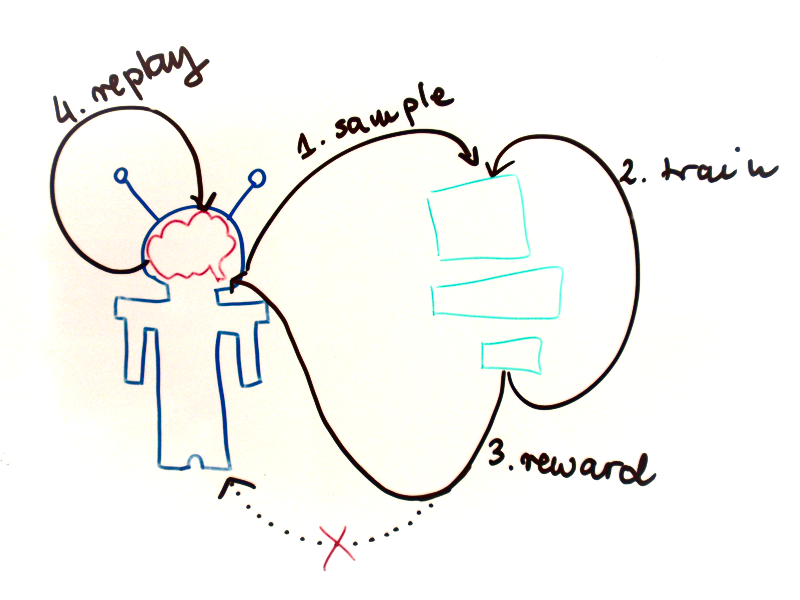
\includegraphics[width=0.85\textwidth]{model.png}

Late architectures (best performing) might not be chosen for replay i.e. not used for  training at all while early architectures (randomly performing) will be overrepresented.
\end{frame}

\begin{frame}{My problem with this paper}
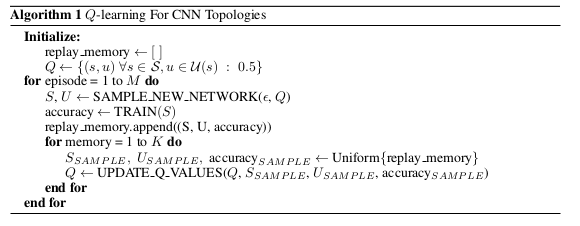
\includegraphics[width=\textwidth]{algorithm-1.png}

Late architectures (best performing) might not be chosen for replay i.e. not used for training at all, while early architectures (randomly performing) will be overrepresented.

\vskip0.1in
\begin{center}
\textbf{WHY?}
\end{center}
\end{frame}


\begin{frame}{Important note}
  \begin{center}
  \Huge{\faLightbulbO}
\end{center}

"While we report results for image classification problems, our method could be applied to different problem settings, including supervised (e.g., classification, regression) and unsupervised (e.g., autoencoders)"
\end{frame}


\begin{frame}{More}
\begin{center}
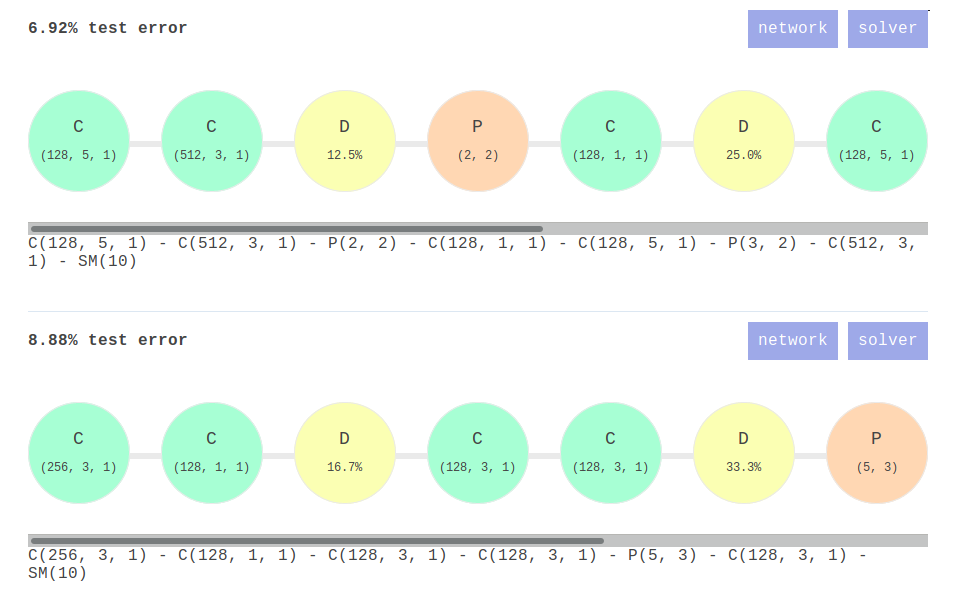
\includegraphics[width=0.8\textwidth]{bowen.png}
\end{center}
\begin{itemize}
\item arXiv 1611.02167 \url{https://arxiv.org/abs/1611.02167}
\item GitHub \url{https://bowenbaker.github.io/metaqnn/}
\end{itemize}
\end{frame}

\end{document}
